%%% Verze pro jednostranný tisk:
\documentclass[11pt,a4paper]{report}
\usepackage[top=25mm,bottom=25mm,right=25mm,left=30mm,head=12.5mm,foot=12.5mm]{geometry}
\let\openright=\clearpage

%%% Pokud tiskneme oboustranně:
%\documentclass[11pt,a4paper,twoside,openright]{report}
%\usepackage[top=25mm,bottom=25mm,right=25mm,left=30mm,head=12.5mm,foot=12.5mm]{geometry}
%\let\openright=\cleardoublepage

%%% DEFINICE ZÁKLADNÍCH PROMĚNNÝCH
\def\TypPrace{DP}
\def\Jazyk{cze}
%\def\Jazyk{eng} % angličtina/english

%%% Definice různých užitečných maker (viz popis uvnitř souboru)
%%% Tento soubor obsahuje definice různých užitečných maker a prostředí %%%
%%% Další makra připisujte sem, ať nepřekáží v ostatních souborech.     %%%
%%% This file contains definitions of various useful macros and environments      %%%
%%% Assign additional macros here so that they do not interfere with other files. %%%

\usepackage{ifpdf}
\usepackage{ifxetex}
\usepackage{ifluatex}

%%% Nastavení pro použití samostatné bibliografické databáze.
%%% Settings for using a separate bibliographic database.
\input biblatex-setup

%% Přepneme na českou sazbu, fonty Latin Modern a kódování češtiny
\ifthenelse{\boolean{xetex}\OR\boolean{luatex}}
{ % use fontspec and OpenType fonts with utf8 engines
	\usepackage[english,slovak,czech]{babel}
	\usepackage[autostyle,english=british,czech=quotes]{csquotes}
	\usepackage{fontspec}
	\defaultfontfeatures{Ligatures=TeX,Scale=MatchLowercase}
}
{
	\usepackage[english,slovak,czech]{babel}
	\usepackage{lmodern}
	\usepackage[T1]{fontenc}
	\usepackage{textcomp}
	\usepackage[utf8]{inputenc}
	\usepackage[autostyle,english=british,czech=quotes]{csquotes}
}
\ifluatex
	\makeatletter
	\let\pdfstrcmp\pdf@strcmp
	\makeatother
\fi

\usepackage[a-2u]{pdfx}     % výsledné PDF bude ve standardu PDF/A-2u
% resulting PDF will be in the PDF / A-2u standard

%%% Další užitečné balíčky (jsou součástí běžných distribucí LaTeXu)
\usepackage{amsmath}        % rozšíření pro sazbu matematiky / extension for math typesetting
\usepackage{amsfonts}       % matematické fonty / mathematical fonts
\usepackage{amssymb}        % symboly / symbols
\usepackage{amsthm}         % sazba vět, definic apod. / typesetting of sentences, definitions, etc.
\usepackage{bm}             % tučné symboly (příkaz \bm) / bold symbols (\bm command)
\usepackage{graphicx}       % vkládání obrázků / graphics inserting
\usepackage{listings}       % vylepšené prostředí pro strojové písmo / improved environment for source codes typesetting
\usepackage{fancyhdr}       % prostředí pohodlnější nastavení hlavy a paty stránek / environment for more comfortable adjustment of the head and foot of the pages
\usepackage{icomma}         % inteligetní čárka v matematickém módu / intelligent comma in math mode
\usepackage{dcolumn}        % lepší zarovnání sloupců v tabulkách / better alignment of columns in tables
\usepackage{booktabs}       % lepší vodorovné linky v tabulkách / better horizontal lines in tables
\usepackage{tabularx}       % vhodné pro tabulky s delšími texty / suitable for tables with longer texts
\usepackage{longtable}      % vhodné pro vícestránkové tabulky / suitable for multi-page tables
\usepackage{dirtree}        % vykreslování adresářových stromů / rendering directory trees
\makeatletter
\@ifpackageloaded{xcolor}{
	\@ifpackagewith{xcolor}{usenames}{}{\PassOptionsToPackage{usenames}{xcolor}}
}{\usepackage[usenames]{xcolor}} % barevná sazba / color typesetting
\makeatother
\usepackage{multicol}       % práce s více sloupci na stránce / work with multiple columns on a page
\usepackage{multirow}
\usepackage{lettrine}
\usepackage{caption}
\usepackage{enumitem}
\setlist[itemize]{noitemsep, topsep=0pt, partopsep=0pt}
\setlist[enumerate]{noitemsep, topsep=0pt, partopsep=0pt}
\setlist[description]{noitemsep, topsep=0pt, partopsep=0pt}

\usepackage{tocloft}
\usepackage{xpatch}
\setlength\cftparskip{0pt}
\setlength\cftbeforechapskip{1.5ex}
\setlength\cftfigindent{0pt}
\setlength\cfttabindent{0pt}
\setlength\cftbeforeloftitleskip{0pt}
\setlength\cftbeforelottitleskip{0pt}
\setlength\cftbeforetoctitleskip{0pt}
\renewcommand{\cftlottitlefont}{\Huge\bfseries\sffamily}
\renewcommand{\cftloftitlefont}{\Huge\bfseries\sffamily}
\renewcommand{\cfttoctitlefont}{\Huge\bfseries\sffamily}

% vyznaceni odstavcu
% differentiation of new paragraphs
\parindent=0pt
\parskip=11pt

% zakaz vdov a sirotku - jednoradkovych pocatku ci koncu odstavcu na prechodu mezi strankami
% Prohibition of widows and orphans - single-line beginning and end of paragraph at the transition between pages
\clubpenalty=1000
\widowpenalty=1000
\displaywidowpenalty=1000

% nastaveni radkovani
% setting of line spacing
\renewcommand{\baselinestretch}{1.20}

% nastaveni pro nadpisy - tucne a bezpatkove
% settings for headings - bold and sans serif
\usepackage{sectsty}
\allsectionsfont{\sffamily}

% nastavení hlavy a paty stránek
% page head and foot settings
\makeatletter
\if@twoside%
	\fancypagestyle{fancyx}{%
		\fancyhf{}
		\fancyhead[RE]{\rightmark}
		\fancyhead[LO]{\leftmark}
		\fancyfoot[RO,LE]{\thepage}
		\renewcommand{\headrulewidth}{.5pt}
		\renewcommand{\footrulewidth}{.5pt}
	}
	\fancypagestyle{plain}{%
		\fancyhf{}
		\fancyfoot[RO,LE]{\thepage}
		\renewcommand{\headrulewidth}{0pt}
		\renewcommand{\footrulewidth}{0.5pt}
	}
\else
	\fancypagestyle{fancyx}{%
		\fancyhf{}
		\fancyhead[R]{\leftmark}
		\fancyfoot[R]{\thepage}
		\renewcommand{\headrulewidth}{.5pt}
		\renewcommand{\footrulewidth}{.5pt}
	}
	\fancypagestyle{plain}{%                       
		\fancyhf{} % clear all header and footer fields
		\fancyfoot[R]{\thepage}
		\renewcommand{\headrulewidth}{0pt}
		\renewcommand{\footrulewidth}{0.5pt}
	}
\fi
\renewcommand*{\cleardoublepage}{\clearpage\if@twoside \ifodd\c@page\else
			\hbox{}%
			\thispagestyle{empty}%
			\newpage%
			\if@twocolumn\hbox{}\newpage\fi\fi\fi
}
\makeatother

% Tato makra přesvědčují mírně ošklivým trikem LaTeX, aby hlavičky kapitol
% sázel příčetněji a nevynechával nad nimi spoustu místa. Směle ignorujte.
% These macros convince with a slightly ugly LaTeX trick to make chapter headers
% bet more sane and didn't miss a lot of space above them. Be boldly ignore it.
\makeatletter
\def\@makechapterhead#1{
	{\parindent \z@ \raggedright \sffamily
		\Huge\bfseries \thechapter. #1
		\par\nobreak
		\vskip 20\p@
	}}
\def\@makeschapterhead#1{
	{\parindent \z@ \raggedright \sffamily
		\Huge\bfseries #1
		\par\nobreak
		\vskip 20\p@
	}}
\makeatother

% Trochu volnější nastavení dělení slov, než je default.
% Slightly looser hyphenation setting than default.
\lefthyphenmin=2
\righthyphenmin=2

% Zapne černé "slimáky" na koncích řádků, které přetekly, abychom si jich lépe všimli.
% Turns on the black "snails" at the ends of the lines that overflowed to get us noticed them better.
\overfullrule=1mm

\def\BibTeX{{\rm B\kern-.05em{\sc i\kern-.025em b}\kern-.08em
		T\kern-.1667em\lower.7ex\hbox{E}\kern-.125emX}}

%% Balíček hyperref, kterým jdou vyrábět klikací odkazy v PDF,
%% ale hlavně ho používáme k uložení metadat do PDF (včetně obsahu).
%% Většinu nastavítek přednastaví balíček pdfx.
%% A hyperref package that can be used to produce clickable links in PDF,
%% but we mainly use it to store metadata in PDF (including content).
%% Most settings are preset by the pdfx package.
\hypersetup{unicode}
\hypersetup{breaklinks=true}
\hypersetup{hidelinks}
%% odkazy barevně
%% links in color
\hypersetup{colorlinks=true,urlcolor=blue}
%% odkazy černě
%% links in black
%% \hypersetup{colorlinks=true,allcolors=black} 

\renewcommand{\UrlBreaks}{\do\/\do\=\do\+\do\-\do\_\do\ \do\a\do\b\do\c\do\d%
	\do\e\do\f\do\g\do\h\do\i\do\j\do\k\do\l\do\m\do\n\do\o\do\p\do\q\do\r\do\s%
	\do\t\do\u\do\v\do\w\do\x\do\y\do\z\do\A\do\B\do\C\do\D\do\E\do\F\do\G\do\H%
	\do\I\do\J\do\K\do\L\do\M\do\N\do\O\do\P\do\Q\do\R\do\S\do\T\do\U\do\V\do\W%
	\do\X\do\Y\do\Z\do\1\do\2\do\3\do\4\do\5\do\6\do\7\do\8\do\9\do\0}
\urlstyle{tt}

%%% Prostředí pro sazbu kódu, případně vstupu/výstupu počítačových
%%% programů. (Vyžaduje balíček listings -- fancy verbatim.)
%%% Environment for source code typesetting, or computer input/output
%%% programs. (Requires package listings - fancy verbatim.)
\lstnewenvironment{code}[3]{\lstset{language=#1, caption=#2, label=#3, basicstyle=\small\ttfamily, numbers=left, xleftmargin=2em, frame=single, framexleftmargin=2em}}{}
\makeatletter
\xpatchcmd\l@lstlisting{1.5em}{0em}{}{}
\makeatother

%%% Úprava formátování popisků obrázků, tabulek a výpisů dle APA7
%%% Change format of captions for figures, tables and extracts according to APA7
\AtBeginEnvironment{figure}{\addvspace{2ex}}
\AtBeginEnvironment{table}{\addvspace{2ex}}
\AtBeginEnvironment{lstlisting}{\addvspace{2ex}}
\AfterEndEnvironment{figure}{\addvspace{1ex}}
\AfterEndEnvironment{table}{\addvspace{1ex}}
\AfterEndEnvironment{lstlisting}{\addvspace{1ex}}
\DeclareCaptionLabelSeparator*{spaced}{\\}
\captionsetup[table]{labelfont=bf,textfont=it,justification=justified,singlelinecheck=false,labelsep=spaced,skip=2ex}
\captionsetup[figure]{labelfont=bf,textfont=it,justification=justified,singlelinecheck=false,labelsep=spaced,skip=1ex}
\captionsetup[lstlisting]{labelfont=bf,textfont=it,justification=justified,singlelinecheck=false,labelsep=spaced,skip=2ex}

%%% Tato část obsahuje texty závislé na typu práce, jazyku a pohlaví %%%
%%% This part contains texts depending on the type of work, language and gender %%%

\newcommand{\ifstringequal}[4]{%
	\ifnum\pdfstrcmp{#1}{#2}=0
		#3%
	\else
		#4%
	\fi
}

\def\TypPraceBP{BAKALÁŘSKÁ PRÁCE}
\def\TypPraceDP{DIPLOMOVÁ PRÁCE}
\def\SeznamZkratek{Seznam použitých zkratek}
\def\Prilohy{Přílohy}
\def\VSE{Vysoká škola ekonomická v Praze}
\def\FIS{Fakulta informatiky a statistiky}
\def\StudijniProgramText{Studijní program}
\def\SpecializaceText{Specializace}
\def\AutorText{Autor}
\def\VedouciText{Vedoucí práce}
\def\KonzultantText{Konzultant práce}
\def\Praha{Praha}
\def\PodekovaniText{Poděkování}
\def\ProhlaseniAIText{Prohlášení o využití umělé inteligence}
\def\bibnamex{Použitá literatura}
\renewcommand*{\lstlistlistingname}{Seznam zdrojových kódů}
\def\lstlistingname{Výpis}

\makeatletter
\ifstringequal{\Jazyk}{eng}{\main@language{english}}{}
\ifstringequal{\Jazyk}{slo}{\main@language{slovak}}{}
\makeatother

\ifstringequal{\Jazyk}{eng}{
	\def\TypPraceBP{BACHELOR THESIS}
	\def\TypPraceDP{MASTER THESIS}
	\def\SeznamZkratek{List of abbreviations}
	\def\Prilohy{Appendices}
	\def\VSE{Prague University of Economics and Business}
	\def\FIS{Faculty of Informatics and Statistics}
	\def\StudijniProgramText{Study program}
	\def\SpecializaceText{Specialization}
	\def\AutorText{Author}
	\def\VedouciText{Supervisor}
	\def\KonzultantText{Consultant}
	\def\Praha{Prague}
	\ifstringequal{\TypPrace}{BP}{\def\Praci{bachelor thesis }}{}
	\ifstringequal{\TypPrace}{DP}{\def\Praci{master thesis }}{}
	\def\PodekovaniText{Acknowledgements}
	\def\ProhlaseniAIText{Declaration on the Use of Artificial Intelligence}
	\def\bibnamex{References}
	\renewcommand*{\lstlistlistingname}{List of source codes}
	\def\lstlistingname{Source code}
	\ifdef{\finalnamedelim}{\renewcommand*{\finalnamedelim}{\addspace and \addspace}}%
}{}

\ifstringequal{\Jazyk}{slo}{
	\def\TypPraceBP{BAKALÁRSKA PRÁCA}
	\def\TypPraceDP{DIPLOMOVÁ PRÁCA}
	\def\SeznamZkratek{Zoznam použitých skratiek}
	\def\Prilohy{Prílohy}
	\def\StudijniProgramText{Študijný program}
	\def\SpecializaceText{Špecializácia}
	\def\VedouciText{Vedúci práce}
	\def\KonzultantText{Konzultant práce}
	\ifstringequal{\TypPrace}{BP}{\def\Praci{bakalársku prácu }}{}
	\ifstringequal{\TypPrace}{DP}{\def\Praci{diplomovú prácu }}{}
	\def\PodekovaniText{Poďakovanie}
	\def\ProhlaseniAIText{Vyhlásenie o využití umelej inteligencie}
	\def\bibnamex{Použitá literatúra}
	\renewcommand*{\lstlistlistingname}{Zoznam zdrojových kódov}
	\def\lstlistingname{Výpis}
}{}

\ifstringequal{\TypPrace}{BP}{\def\TypPraceText{\TypPraceBP}}{}
\ifstringequal{\TypPrace}{DP}{\def\TypPraceText{\TypPraceDP}}{}

% todomt command for 
\usepackage[most]{tcolorbox}
\usepackage{xcolor}

\newcounter{todo}

\newtcolorbox{todobox}[1]{
	enhanced,
	breakable,
	colback=red!7,
	colframe=red!80!black,
	coltitle=white,
	colbacktitle=red!80!black,
	title={\textbf{TODO (\thetodo): #1}},
	fonttitle=\bfseries\large,
	boxrule=1.5pt,
	arc=2mm,
	left=4mm,
	right=4mm,
	top=3mm,
	bottom=3mm,
	before skip=5mm,
	after skip=5mm
}

\newcommand{\todo}[2]{
	\refstepcounter{todo}
	\begin{todobox}{#1}
		#2
	\end{todobox}
}

\def\NazevPrace{Redesign uživatelského rozhraní aplikace pro správu pracovního prostředí}
\def\AutorPrace{Bc. Vojtěch Nerad}
\def\DatumOdevzdani{prosinec 2026}
\def\Vedouci{Ing. Tereza Werdan Zichová, Ph.D.}
\def\Konzultant{[jméno a příjmení konzultanta vč. titulů]}
\def\StudijniProgram{Informační systémy a technologie}
\def\Specializace{UX výzkum a design}

%%% Nepovinné poděkování (vedoucímu práce, konzultantovi, tomu, kdo zapůjčil software, literaturu apod.)
%%% Optional thanks (the supervisor, the consultant, the borrower of software, literature, etc.)
\def\Podekovani{%
Poděkování.
}

%%% Abstrakt (doporučený rozsah cca 150-250 slov; nejedná se o zadání práce)
\def\Abstrakt{%
Diplomová práce se zabývá návrhem redesignu uživatelského rozhraní existující aplikace určené pro správu pracovního prostředí (workplace management).
Aplikace vznikala postupně jako interní nástroj podporující provozní procesy a její vývoj se soustředil primárně na funkčnost,
nikoliv na vizuální podobu či konzistentní uživatelskou zkušenost.
V důsledku neřízeného vývoje se rozhraní stalo nekoherentním a pro uživatele obtížně srozumitelným.
Cílem práce je navrhnout a ověřit nový uživatelský design, který zvýší přehlednost,
intuitivnost a vizuální konzistenci rozhraní, a současně umožní budoucí škálování systému.
Práce vychází z metod uživatelsky orientovaného designu a kombinuje uživatelský výzkum,
analýzu stávajícího řešení a návrh design systému.
Následně byly vytvořeny interaktivní prototypy, které byly iterativně testovány s uživateli.
Výstupem je ucelený návrh redesignu klíčových obrazovek připravený k implementaci,
design systém a doporučení pro další rozvoj aplikace.
Tyto výstupy prokazatelně zlepšují uživatelskou zkušenost a tvoří systematický základ pro budoucí rozšiřování nástroje.
}
\def\AbstraktEN{
This master’s thesis focuses on redesigning the user interface of an existing workplace management application. The application was gradually developed as an internal tool supporting operational processes, with development focused primarily on functionality rather than visual design or a consistent user experience. As a result of this uncontrolled development, the interface became incoherent and difficult for users to understand.
The aim of the thesis is to design and validate a new user interface that improves the clarity, intuitiveness, and visual consistency of the application while also enabling future system scalability. The work is based on user-centered design methods and combines user research, an analysis of the existing solution, and the design of a design system. Interactive prototypes were subsequently created and iteratively tested with users.
The outcome is a comprehensive redesign of key screens, prepared for implementation, together with a design system and recommendations for the further development of the application. These outcomes demonstrably improve the user experience and provide a systematic foundation for the future expansion of the tool.

}

%%% 3 až 5 klíčových slov (doporučeno)
\def\KlicovaSlova{redesign uživatelského rozhraní, uživatelská zkušenost (UX), workplace management, uživatelský výzkum, design systém}
\def\KlicovaSlovaEN{user interface redesign, user experience (UX), workplace management, user research, design system}

%%% Titulní strana a různé povinné informativní strany
\begin{document}
%%% Titulní strana práce a další povinné informační strany

%%% Titulní strana práce

\pagestyle{empty}
\hypersetup{pageanchor=false}

\begin{center}
\Huge\sffamily
\VSE\\
\FIS

\vspace{\stretch{1}}

\ifstringequal{\Jazyk}{eng}{
	
\includegraphics[width=.5\textwidth]{img/FIS_2_logo_2_rgb_EN}
}{
	
\includegraphics[width=.5\textwidth]{img/FIS_2_logo_2_rgb_CZ}
}

\vspace{\stretch{2}}

\bfseries\NazevPrace

\vspace{8mm}
\mdseries\TypPraceText

\vspace{8mm}
\large
\begin{tabular}{rl}
\StudijniProgramText: & \StudijniProgram \\
\ifthenelse{\equal{\Specializace}{}}{%
	% empty value
	}{
	\rule{0pt}{6mm}%
	\SpecializaceText: & \Specializace \\
}
\end{tabular}

\vspace{\stretch{8}}

\begin{tabular}{rl}
\AutorText: & \AutorPrace \\
\noalign{\vspace{2mm}}
\VedouciText: & \Vedouci \\
\ifthenelse{\equal{\Konzultant}{}}{%
	% empty value
	}{
	\rule{0pt}{6mm}%
	\KonzultantText: & \Konzultant \\
}
\end{tabular}

\vspace{8mm}
\Praha, \DatumOdevzdani
\end{center}


%%% Prohlášení k použití AI
\hypersetup{pageanchor=true}
\cleardoublepage
\pagestyle{plain}
\openright
\vspace*{\fill}
\section*{\ProhlaseniAIText}
\noindent

\ifstringequal{\Jazyk}{cze}{
\textit{NEHODÍCÍ SE SMAŽTE (STEJNĚ JAKO TUTO VĚTU A ČÍSLOVÁNÍ ODSTAVCŮ)
\textbf{ -- změny proveďte v souboru \texttt{prohlaseniAI.tex} v řádcích 10--36}.}

1) Při zpracování předložené práce \textbf{nebyly použity} žádné nástroje umělé inteligence.

2) Potvrzuji, že při přípravě předložené práce \textbf{byly použity} nástroje umělé inteligence. Konkrétně byly použity těmito způsoby:
\begin{itemize}
\item zlepšení gramatiky a jazykového stylu, 
\item vyhledávání a shrnutí literatury,
\item úprava a rozšíření textových částí,
\item generování části zdrojových kódů,
\item generování dat,
\item generování obrázků a jiných médií,
\item jiným způsobem (uveďte).
\end{itemize}

{\leftskip=1.5em
Každé použití některého ze způsobů je samostatně dokumentováno v příloze práce, 
kde je uvedeno podrobnější vysvětlení -- který nástroj byl ve které části práce 
konkrétně použit; je zvýrazněn vlastní přínos.

Potvrzuji, že:
\begin{itemize}
\item má práce je originální a byla zpracována v souladu s etickými standardy, zejména s Etickým kodexem Vysoké školy ekonomické v Praze, že jsou v práci citovány všechny použité informační zdroje a že generovaný obsah byl mnou ověřen;
\item přijímám plnou odpovědnost za celý obsah závěrečné práce.
\end{itemize}
}
}{}


\ifstringequal{\Jazyk}{eng}{
\textit{DELETE WHAT DOES NOT APPLY (AS WELL AS THIS SENTENCE AND PARAGRAPH NUMBERING)
\textbf{ -- changes must be made in the \texttt{prohlaseniAI.tex} file in lines 41--69}.}

1) No artificial intelligence tools were used in the preparation of the submitted work.

2) I confirm that artificial intelligence tools were used in the preparation of 
the submitted work. Specifically, they were used in the following ways:

\begin{itemize}
\item improvement of grammar and language style,
\item searching for and summarizing literature,
\item editing and expanding textual sections,
\item generation of parts of source code,
\item data generation,
\item generation of images and other media,
\item other (please specify).
\end{itemize}

{\leftskip=1.5em
Each use of any of the above methods is separately documented in an appendix to 
the thesis, which provides a more detailed explanation of which tool was used in 
which specific part of the work; the author's own contribution is highlighted.

I confirm that:
\begin{itemize}
\item my work is original and was prepared in accordance with ethical standards, in particular the Code of Ethics of the Prague University of Economics and Business; that all information sources used are properly cited in the work; and that any generated content has been verified by me;
\item I accept full responsibility for the entire content of the thesis. 
\end{itemize}
}
}{}


\ifstringequal{\Jazyk}{slo}{
\textit{NEHODIACI SA ZMAŽTE (ROVNAKO AKO TÚTO VETU A ČÍSLOVANIE ODSTAVCOV)
\textbf{ -- zmeny vykonajte v súbore \texttt{prohlaseniAI.tex} v riadkoch 74--100}.}

1) Pri spracovaní predloženej práce \textbf{neboli použité} žiadne nástroje umelej inteligencie.

2) Potvrdzujem, že pri príprave predloženej práce \textbf{boli použité} nástroje umelej inteligencie. Konkrétne boli použité týmito spôsobmi:
\begin{itemize}
\item zlepšenie gramatiky a jazykového štýlu,
\item vyhľadávanie a zhrnutie literatúry,
\item úprava a rozšírenie textových častí,
\item generovanie časti zdrojových kódov,
\item generovanie dát,
\item generovanie obrázkov a iných médií,
\item iným spôsobom (uveďte).
\end{itemize}

{\leftskip=1.5em
Každé použitie niektorého zo spôsobov je samostatne dokumentované v prílohe práce,
kde je uvedené podrobnejšie vysvetlenie - ktorý nástroj bol v ktorej časti práce
konkrétne použitý; je zvýraznený vlastný prínos.

Potvrdzujem, že:
\begin{itemize}
\item moja práca je originálna a bola spracovaná v súlade etickými štandardmi, najmä s Etickým kódexom Vysokej školy ekonomickej v Prahe, že sú v práci citované všetky použité informačné zdroje a že generovaný obsah bol mnou overený;
\item prijímam plnú zodpovednosť za celý obsah záverečnej práce.
\end{itemize}
}
}{}

\vspace{1cm}



%%% Poděkování
\hypersetup{pageanchor=true}
\cleardoublepage
\pagestyle{plain}
\openright
\vspace*{\fill}
\section*{\PodekovaniText}
\noindent
\Podekovani
\vspace{1cm}


%%% Povinná informační strana práce
\openright
\section*{Abstrakt}
\noindent
\Abstrakt
\subsection*{Klíčová slova}
\noindent
\KlicovaSlova

\bigskip\bigskip\bigskip\bigskip\bigskip
\section*{Abstract}
\noindent
\AbstraktEN
\subsection*{Keywords}
\noindent
\KlicovaSlovaEN

\openright


%%% Strana s automaticky generovaným obsahem práce
\setcounter{tocdepth}{2}
\tableofcontents

%%% Seznam obrázků v práci
\openright
\listoffigures
Poznámka: Seznam obrázků je vhodné použít, pokud počet obrázků v textu práce je větší než 20.

%%% Seznam tabulek v práci (volitelně)
\clearpage
\listoftables
Poznámka: Seznam tabulek je vhodný použít, pokud počet tabulek v textu práce je větší než 20.

%%% Seznam zdrojových kódů v práci (volitelně)
\clearpage
\lstlistoflistings
Poznámka: Seznam výpisů programového kódu je vhodné použít, pokud počet vložených objektů tohoto typu je větší než 20. 

%%% Seznam zkratek v práci (volitelně)
\chapter*{\SeznamZkratek}

\begin{multicols}{2}
\raggedright
\begin{description}
\item [BCC] Blind Carbon Copy
\item [CC] Carbon Copy
\item [CERT] Computer Emergency Response Team
\item [CSS] Cascading Styleheets
\item [DOI] Digital Object Identifier
\item [HTML] Hypertext Markup Language
\item [REST] Representational State Transfer
\item [SOAP] Simple Object Access Protocol
\item [URI] Uniform Resource Identifier
\item [URL] Uniform Resource Locator
\item [XML] eXtended Markup Language
\end{description}
\end{multicols}

Poznámka: Seznam zkratek je vhodný použít, pokud počet zkratek v textu práce je větší než 20 a nejedná se o zkratky běžné. Každou zkratku je třeba při jejím prvním použití vymezit, např.: „Pro zkoumání závislosti jsme použili regresní analýzu, konkrétně zobecněné lineární modely (\emph{generalized linear models}, GLM).“

\pagestyle{fancyx}
%%% Jednotlivé kapitoly práce jsou pro přehlednost uloženy v samostatných souborech
{%
\pagestyle{plain}
\chapter*{Doporučení pro tvorbu závěrečných prací na FIS}

\begin{quote}
\bfseries\itshape
Tato část šablony nepatří standardně do bakalářské/diplomové práce. Pro finální 
text je zapotřebí:
\begin{itemize}
\item smazat v souboru \verb|prace.tex| řádek \verb|\chapter*{Doporučení pro tvorbu závěrečných prací na FIS}

\begin{quote}
\bfseries\itshape
Tato část šablony nepatří standardně do bakalářské/diplomové práce. Pro finální 
text je zapotřebí:
\begin{itemize}
\item smazat v souboru \verb|prace.tex| řádek \verb|\chapter*{Doporučení pro tvorbu závěrečných prací na FIS}

\begin{quote}
\bfseries\itshape
Tato část šablony nepatří standardně do bakalářské/diplomové práce. Pro finální 
text je zapotřebí:
\begin{itemize}
\item smazat v souboru \verb|prace.tex| řádek \verb|\include{doporuceni}|
\item  a případně též pak zbytečný soubor \verb|doporuceni.tex|.
\end{itemize}
\end{quote}

Následující doporučení pro tvorbu závěrečných prací (dále jen „doporučení“) jsou 
určena k hodnocení obhajitelnosti závěrečné práce. Jsou určena pro všechny typy 
závěrečných prací na všech bakalářských a magisterských studijních programech. 
Nenahrazují posudky k závěrečné práci. Pokud komise považuje závěrečnou práci za 
neobhajitelnou, měla by argumentovat nesplněním některé položky z těchto 
doporučení.

\subsection*{Odvedená práce}
\begin{itemize}
\item \vspace*{-2ex}Student provedl odbornou práci v oblasti studijního programu, který studuje (včetně interdisciplinárních oblastí).
\item Závěrečná práce prokazuje studentovu orientaci ve zvolené oblasti a jeho schopnost v této oblasti definovat a splnit zvolený cíl. 
\item Je zřejmé, že student odvedl odbornou práci o pracnosti v rozsahu měsíců.
\end{itemize}

\subsection*{Cíle a kontext}
\begin{itemize}
\item \vspace*{-2ex}V textu závěrečné práce jsou popsána východiska – odborný kontext, ze kterého student vychází – situace v odborném poznání nebo situace v konkrétním aplikačním případě.
\item Východiska obsahují jen poznatky, které mají vliv na výsledky závěrečné práce.
\item V textu závěrečné práce je zřetelně popsán cíl, kterého má závěrečná práce dosáhnout; pokud je cílem řešení problému, je tento problém dostatečně vymezen.
\item Je argumentována smysluplnost cílů ve vztahu k východiskům.
\item V textu je argumentována specifičnost hlavního cíle – nejde o generický, mnohokrát zcela stejně řešený problém.
\item Formulace cíle se vztahuje k nějakému odbornému problému, nikoli k textu závěrečné práce samotné, ke čtenáři ani k autorovi. Tedy cíl není formulován jako „napsat text“, „sdělit čtenáři“, „popsat problematiku“, „vysvětlit“, „seznámit se s literaturou z oblasti” apod.
\item Text závěrečné práce je odborný, nikoli populárně naučný. Řeší odborný (praktický nebo teoretický) problém.
\end{itemize}

\subsection*{Metodika}
\begin{itemize}
\item \vspace*{-2ex}Text závěrečné práce popisuje postup, podle kterého student pracoval, a to odděleně od výsledků.
\item Postup je popsán v krocích, ze kterých lze odhadnout jejich pracnost.
\item Postup uvádí veškerou práci, kterou student provedl. Pokud jsou v postupu uvedeny kroky, které student neprovedl, jsou tak zřetelně označeny (a je uveden důvod).
\item Postup je popsán tak, že pokud by podle něj postupoval někdo jiný, došel by k obdobným výsledkům jako student.
\item Postup je popsán konkrétně, nikoli jen pomocí obecných názvů myšlenkových postupů typu analýza, dedukce, syntéza apod.
\item Pokud je použit postup podle zavedených a v literatuře popsaných metod, není nutné vysvětlovat detailně jejich fungování. Student by měl ale zdůvodnit svou volbu použitých metod, případně popsat odchylky skutečného postupu oproti zavedeným metodám.
\end{itemize}

\subsection*{Výsledky}
\begin{itemize}
\item \vspace*{-2ex}Výsledky prokazují, že student provedl odbornou práci v oblasti studijního programu, který studuje (včetně interdisciplinárních oblastí).
\item Z formulace textu závěrečné práce je zřejmé, co je původním výsledkem studenta, co faktem přebíraným ze zdrojů a co spekulací, resp. diskusí výsledků.
\item Text popisuje a interpretuje výsledky v souladu s postupem.
\item V textu jsou popsány dílčí výsledky jako výstupy jednotlivých kroků. Méně důležité výsledky jsou uvedeny v přílohách, takže text zůstává přehledný.
\item Je doloženo provedení jednotlivých kroků (např. výpočty, popisná statistika, záznamy z rozhovorů, programový kód, deník výzkumníka apod.), např. nahráním příloh do InSIS.
\item Text závěrečné práce popisuje odborné výsledky v logicky navazujícím argumentačním toku. 
\end{itemize}

\subsection*{Závěry}
\begin{itemize}
\item \vspace*{-2ex}Závěry hodnotí míru naplnění cíle.
\item Závěry argumentují, jak výsledky přispěly k vyřešení problému.
\item Závěry popisují, jaký je možný vliv výsledků na kontext (situaci v odborném prostředí nebo v konkrétním aplikačním případě), např. možné další pokračování práce.
\item Závěry zmiňují možná omezení dosažených výsledků.
\end{itemize}

\subsection*{Originalita}
\begin{itemize}
\item \vspace*{-2ex}Veškeré převzaté, přeložené nebo parafrázované texty jsou řádně označeny a citovány v souladu s citační normou APA 7 (doporučujeme využívat citační nástroj Zotero).
\item V případě použití nástrojů pro automatické generování textů je toto použití v souladu s pravidly a metodickými doporučeními na VŠE.
\item Text závěrečné práce cituje a parafrázuje pouze zdroje, které byly použity pro řešení problému, nebo vymezení kontextu.
\item Text závěrečné práce zbytečně nerekapituluje zřejmé teoretické poznatky (např. ze základních kurzů studijního programu).
\item Pokud student ve výjimečných případech nepracoval zcela sám, jsou u jednotlivých kroků postupu nebo formou tabulky v příloze uvedeni spolupracovníci (firemní, akademičtí) a podíl studenta na jejich provedení.
\end{itemize}

\subsection*{Forma}
\begin{itemize}
\item \vspace*{-2ex}Text závěrečné práce je psán jako ucelený souvislý strukturovaný text, jako odstavce členěné do kapitol, ve struktuře vhodné pro řešený problém.
\item Stránky, tabulky, obrázky, přílohy (apod.) jsou číslovány.
\item V závěrečné práci se nevyskytují tabulky, obrázky, přílohy, programový kód (apod.), které nejsou odkazovány ze souvislého textu.
\item Forma závěrečné práce je v souladu s doporučeními zpřístupněnými na intranetu pro studenty FIS.
\item Závěrečná práce může mít formu vědeckého článku. V takovém případě může být doplněna vysvětlujícím úvodem (např. popis časopisu, průběh recenzního řízení, spoluautorství vedoucího závěrečné práce apod.).
\end{itemize}

\subsection*{Doplňující nároky pro diplomovou práci}
\begin{itemize}
\item \vspace*{-2ex}Diplomová práce významně prohlubuje oblast poznání v daném tématu.
\item V diplomové práci je jasně specifikován vlastní přínos autora, který je v souladu s cíli práce. 
\item Je nutné provést validaci výsledků diplomové práce (např. srovnání dosažených výsledků s literaturou, matematický důkaz, strukturované rozhovory se zájmovými skupinami, exaktní testování/měření výsledků apod.).
\end{itemize}

\subsection*{Specifika týmových závěrečných prací}
\begin{itemize}
\item \vspace*{-2ex}Skutečnost, že bude závěrečná práce realizována v týmu, musí být uvedena v Zadání závěrečné práce uloženém v InSISu, a tedy schválena vedoucím práce a garantem studijního programu (specializace).
\item Každý student z týmu odevzdává individuální závěrečnou práci, která je individuálně posuzována, individuálně obhajována a hodnocena. Každý student je odpovědný za celý text závěrečné práce.
\item Pouze malá část závěrečné práce může být ve vedoucím závěrečné práce schválených případech společná. Více než 70 % závěrečné práce je individuální.
\item V týmu vytvářené artefakty by měly být publikovány například v Git nebo na wiki projektu a autoři závěrečných prací na ně odkazují.
\item Každá v týmu realizovaná závěrečná práce obsahuje přílohu s názvem Podíl členů týmu na výsledku.
\end{itemize}
|
\item  a případně též pak zbytečný soubor \verb|doporuceni.tex|.
\end{itemize}
\end{quote}

Následující doporučení pro tvorbu závěrečných prací (dále jen „doporučení“) jsou 
určena k hodnocení obhajitelnosti závěrečné práce. Jsou určena pro všechny typy 
závěrečných prací na všech bakalářských a magisterských studijních programech. 
Nenahrazují posudky k závěrečné práci. Pokud komise považuje závěrečnou práci za 
neobhajitelnou, měla by argumentovat nesplněním některé položky z těchto 
doporučení.

\subsection*{Odvedená práce}
\begin{itemize}
\item \vspace*{-2ex}Student provedl odbornou práci v oblasti studijního programu, který studuje (včetně interdisciplinárních oblastí).
\item Závěrečná práce prokazuje studentovu orientaci ve zvolené oblasti a jeho schopnost v této oblasti definovat a splnit zvolený cíl. 
\item Je zřejmé, že student odvedl odbornou práci o pracnosti v rozsahu měsíců.
\end{itemize}

\subsection*{Cíle a kontext}
\begin{itemize}
\item \vspace*{-2ex}V textu závěrečné práce jsou popsána východiska – odborný kontext, ze kterého student vychází – situace v odborném poznání nebo situace v konkrétním aplikačním případě.
\item Východiska obsahují jen poznatky, které mají vliv na výsledky závěrečné práce.
\item V textu závěrečné práce je zřetelně popsán cíl, kterého má závěrečná práce dosáhnout; pokud je cílem řešení problému, je tento problém dostatečně vymezen.
\item Je argumentována smysluplnost cílů ve vztahu k východiskům.
\item V textu je argumentována specifičnost hlavního cíle – nejde o generický, mnohokrát zcela stejně řešený problém.
\item Formulace cíle se vztahuje k nějakému odbornému problému, nikoli k textu závěrečné práce samotné, ke čtenáři ani k autorovi. Tedy cíl není formulován jako „napsat text“, „sdělit čtenáři“, „popsat problematiku“, „vysvětlit“, „seznámit se s literaturou z oblasti” apod.
\item Text závěrečné práce je odborný, nikoli populárně naučný. Řeší odborný (praktický nebo teoretický) problém.
\end{itemize}

\subsection*{Metodika}
\begin{itemize}
\item \vspace*{-2ex}Text závěrečné práce popisuje postup, podle kterého student pracoval, a to odděleně od výsledků.
\item Postup je popsán v krocích, ze kterých lze odhadnout jejich pracnost.
\item Postup uvádí veškerou práci, kterou student provedl. Pokud jsou v postupu uvedeny kroky, které student neprovedl, jsou tak zřetelně označeny (a je uveden důvod).
\item Postup je popsán tak, že pokud by podle něj postupoval někdo jiný, došel by k obdobným výsledkům jako student.
\item Postup je popsán konkrétně, nikoli jen pomocí obecných názvů myšlenkových postupů typu analýza, dedukce, syntéza apod.
\item Pokud je použit postup podle zavedených a v literatuře popsaných metod, není nutné vysvětlovat detailně jejich fungování. Student by měl ale zdůvodnit svou volbu použitých metod, případně popsat odchylky skutečného postupu oproti zavedeným metodám.
\end{itemize}

\subsection*{Výsledky}
\begin{itemize}
\item \vspace*{-2ex}Výsledky prokazují, že student provedl odbornou práci v oblasti studijního programu, který studuje (včetně interdisciplinárních oblastí).
\item Z formulace textu závěrečné práce je zřejmé, co je původním výsledkem studenta, co faktem přebíraným ze zdrojů a co spekulací, resp. diskusí výsledků.
\item Text popisuje a interpretuje výsledky v souladu s postupem.
\item V textu jsou popsány dílčí výsledky jako výstupy jednotlivých kroků. Méně důležité výsledky jsou uvedeny v přílohách, takže text zůstává přehledný.
\item Je doloženo provedení jednotlivých kroků (např. výpočty, popisná statistika, záznamy z rozhovorů, programový kód, deník výzkumníka apod.), např. nahráním příloh do InSIS.
\item Text závěrečné práce popisuje odborné výsledky v logicky navazujícím argumentačním toku. 
\end{itemize}

\subsection*{Závěry}
\begin{itemize}
\item \vspace*{-2ex}Závěry hodnotí míru naplnění cíle.
\item Závěry argumentují, jak výsledky přispěly k vyřešení problému.
\item Závěry popisují, jaký je možný vliv výsledků na kontext (situaci v odborném prostředí nebo v konkrétním aplikačním případě), např. možné další pokračování práce.
\item Závěry zmiňují možná omezení dosažených výsledků.
\end{itemize}

\subsection*{Originalita}
\begin{itemize}
\item \vspace*{-2ex}Veškeré převzaté, přeložené nebo parafrázované texty jsou řádně označeny a citovány v souladu s citační normou APA 7 (doporučujeme využívat citační nástroj Zotero).
\item V případě použití nástrojů pro automatické generování textů je toto použití v souladu s pravidly a metodickými doporučeními na VŠE.
\item Text závěrečné práce cituje a parafrázuje pouze zdroje, které byly použity pro řešení problému, nebo vymezení kontextu.
\item Text závěrečné práce zbytečně nerekapituluje zřejmé teoretické poznatky (např. ze základních kurzů studijního programu).
\item Pokud student ve výjimečných případech nepracoval zcela sám, jsou u jednotlivých kroků postupu nebo formou tabulky v příloze uvedeni spolupracovníci (firemní, akademičtí) a podíl studenta na jejich provedení.
\end{itemize}

\subsection*{Forma}
\begin{itemize}
\item \vspace*{-2ex}Text závěrečné práce je psán jako ucelený souvislý strukturovaný text, jako odstavce členěné do kapitol, ve struktuře vhodné pro řešený problém.
\item Stránky, tabulky, obrázky, přílohy (apod.) jsou číslovány.
\item V závěrečné práci se nevyskytují tabulky, obrázky, přílohy, programový kód (apod.), které nejsou odkazovány ze souvislého textu.
\item Forma závěrečné práce je v souladu s doporučeními zpřístupněnými na intranetu pro studenty FIS.
\item Závěrečná práce může mít formu vědeckého článku. V takovém případě může být doplněna vysvětlujícím úvodem (např. popis časopisu, průběh recenzního řízení, spoluautorství vedoucího závěrečné práce apod.).
\end{itemize}

\subsection*{Doplňující nároky pro diplomovou práci}
\begin{itemize}
\item \vspace*{-2ex}Diplomová práce významně prohlubuje oblast poznání v daném tématu.
\item V diplomové práci je jasně specifikován vlastní přínos autora, který je v souladu s cíli práce. 
\item Je nutné provést validaci výsledků diplomové práce (např. srovnání dosažených výsledků s literaturou, matematický důkaz, strukturované rozhovory se zájmovými skupinami, exaktní testování/měření výsledků apod.).
\end{itemize}

\subsection*{Specifika týmových závěrečných prací}
\begin{itemize}
\item \vspace*{-2ex}Skutečnost, že bude závěrečná práce realizována v týmu, musí být uvedena v Zadání závěrečné práce uloženém v InSISu, a tedy schválena vedoucím práce a garantem studijního programu (specializace).
\item Každý student z týmu odevzdává individuální závěrečnou práci, která je individuálně posuzována, individuálně obhajována a hodnocena. Každý student je odpovědný za celý text závěrečné práce.
\item Pouze malá část závěrečné práce může být ve vedoucím závěrečné práce schválených případech společná. Více než 70 % závěrečné práce je individuální.
\item V týmu vytvářené artefakty by měly být publikovány například v Git nebo na wiki projektu a autoři závěrečných prací na ně odkazují.
\item Každá v týmu realizovaná závěrečná práce obsahuje přílohu s názvem Podíl členů týmu na výsledku.
\end{itemize}
|
\item  a případně též pak zbytečný soubor \verb|doporuceni.tex|.
\end{itemize}
\end{quote}

Následující doporučení pro tvorbu závěrečných prací (dále jen „doporučení“) jsou 
určena k hodnocení obhajitelnosti závěrečné práce. Jsou určena pro všechny typy 
závěrečných prací na všech bakalářských a magisterských studijních programech. 
Nenahrazují posudky k závěrečné práci. Pokud komise považuje závěrečnou práci za 
neobhajitelnou, měla by argumentovat nesplněním některé položky z těchto 
doporučení.

\subsection*{Odvedená práce}
\begin{itemize}
\item \vspace*{-2ex}Student provedl odbornou práci v oblasti studijního programu, který studuje (včetně interdisciplinárních oblastí).
\item Závěrečná práce prokazuje studentovu orientaci ve zvolené oblasti a jeho schopnost v této oblasti definovat a splnit zvolený cíl. 
\item Je zřejmé, že student odvedl odbornou práci o pracnosti v rozsahu měsíců.
\end{itemize}

\subsection*{Cíle a kontext}
\begin{itemize}
\item \vspace*{-2ex}V textu závěrečné práce jsou popsána východiska – odborný kontext, ze kterého student vychází – situace v odborném poznání nebo situace v konkrétním aplikačním případě.
\item Východiska obsahují jen poznatky, které mají vliv na výsledky závěrečné práce.
\item V textu závěrečné práce je zřetelně popsán cíl, kterého má závěrečná práce dosáhnout; pokud je cílem řešení problému, je tento problém dostatečně vymezen.
\item Je argumentována smysluplnost cílů ve vztahu k východiskům.
\item V textu je argumentována specifičnost hlavního cíle – nejde o generický, mnohokrát zcela stejně řešený problém.
\item Formulace cíle se vztahuje k nějakému odbornému problému, nikoli k textu závěrečné práce samotné, ke čtenáři ani k autorovi. Tedy cíl není formulován jako „napsat text“, „sdělit čtenáři“, „popsat problematiku“, „vysvětlit“, „seznámit se s literaturou z oblasti” apod.
\item Text závěrečné práce je odborný, nikoli populárně naučný. Řeší odborný (praktický nebo teoretický) problém.
\end{itemize}

\subsection*{Metodika}
\begin{itemize}
\item \vspace*{-2ex}Text závěrečné práce popisuje postup, podle kterého student pracoval, a to odděleně od výsledků.
\item Postup je popsán v krocích, ze kterých lze odhadnout jejich pracnost.
\item Postup uvádí veškerou práci, kterou student provedl. Pokud jsou v postupu uvedeny kroky, které student neprovedl, jsou tak zřetelně označeny (a je uveden důvod).
\item Postup je popsán tak, že pokud by podle něj postupoval někdo jiný, došel by k obdobným výsledkům jako student.
\item Postup je popsán konkrétně, nikoli jen pomocí obecných názvů myšlenkových postupů typu analýza, dedukce, syntéza apod.
\item Pokud je použit postup podle zavedených a v literatuře popsaných metod, není nutné vysvětlovat detailně jejich fungování. Student by měl ale zdůvodnit svou volbu použitých metod, případně popsat odchylky skutečného postupu oproti zavedeným metodám.
\end{itemize}

\subsection*{Výsledky}
\begin{itemize}
\item \vspace*{-2ex}Výsledky prokazují, že student provedl odbornou práci v oblasti studijního programu, který studuje (včetně interdisciplinárních oblastí).
\item Z formulace textu závěrečné práce je zřejmé, co je původním výsledkem studenta, co faktem přebíraným ze zdrojů a co spekulací, resp. diskusí výsledků.
\item Text popisuje a interpretuje výsledky v souladu s postupem.
\item V textu jsou popsány dílčí výsledky jako výstupy jednotlivých kroků. Méně důležité výsledky jsou uvedeny v přílohách, takže text zůstává přehledný.
\item Je doloženo provedení jednotlivých kroků (např. výpočty, popisná statistika, záznamy z rozhovorů, programový kód, deník výzkumníka apod.), např. nahráním příloh do InSIS.
\item Text závěrečné práce popisuje odborné výsledky v logicky navazujícím argumentačním toku. 
\end{itemize}

\subsection*{Závěry}
\begin{itemize}
\item \vspace*{-2ex}Závěry hodnotí míru naplnění cíle.
\item Závěry argumentují, jak výsledky přispěly k vyřešení problému.
\item Závěry popisují, jaký je možný vliv výsledků na kontext (situaci v odborném prostředí nebo v konkrétním aplikačním případě), např. možné další pokračování práce.
\item Závěry zmiňují možná omezení dosažených výsledků.
\end{itemize}

\subsection*{Originalita}
\begin{itemize}
\item \vspace*{-2ex}Veškeré převzaté, přeložené nebo parafrázované texty jsou řádně označeny a citovány v souladu s citační normou APA 7 (doporučujeme využívat citační nástroj Zotero).
\item V případě použití nástrojů pro automatické generování textů je toto použití v souladu s pravidly a metodickými doporučeními na VŠE.
\item Text závěrečné práce cituje a parafrázuje pouze zdroje, které byly použity pro řešení problému, nebo vymezení kontextu.
\item Text závěrečné práce zbytečně nerekapituluje zřejmé teoretické poznatky (např. ze základních kurzů studijního programu).
\item Pokud student ve výjimečných případech nepracoval zcela sám, jsou u jednotlivých kroků postupu nebo formou tabulky v příloze uvedeni spolupracovníci (firemní, akademičtí) a podíl studenta na jejich provedení.
\end{itemize}

\subsection*{Forma}
\begin{itemize}
\item \vspace*{-2ex}Text závěrečné práce je psán jako ucelený souvislý strukturovaný text, jako odstavce členěné do kapitol, ve struktuře vhodné pro řešený problém.
\item Stránky, tabulky, obrázky, přílohy (apod.) jsou číslovány.
\item V závěrečné práci se nevyskytují tabulky, obrázky, přílohy, programový kód (apod.), které nejsou odkazovány ze souvislého textu.
\item Forma závěrečné práce je v souladu s doporučeními zpřístupněnými na intranetu pro studenty FIS.
\item Závěrečná práce může mít formu vědeckého článku. V takovém případě může být doplněna vysvětlujícím úvodem (např. popis časopisu, průběh recenzního řízení, spoluautorství vedoucího závěrečné práce apod.).
\end{itemize}

\subsection*{Doplňující nároky pro diplomovou práci}
\begin{itemize}
\item \vspace*{-2ex}Diplomová práce významně prohlubuje oblast poznání v daném tématu.
\item V diplomové práci je jasně specifikován vlastní přínos autora, který je v souladu s cíli práce. 
\item Je nutné provést validaci výsledků diplomové práce (např. srovnání dosažených výsledků s literaturou, matematický důkaz, strukturované rozhovory se zájmovými skupinami, exaktní testování/měření výsledků apod.).
\end{itemize}

\subsection*{Specifika týmových závěrečných prací}
\begin{itemize}
\item \vspace*{-2ex}Skutečnost, že bude závěrečná práce realizována v týmu, musí být uvedena v Zadání závěrečné práce uloženém v InSISu, a tedy schválena vedoucím práce a garantem studijního programu (specializace).
\item Každý student z týmu odevzdává individuální závěrečnou práci, která je individuálně posuzována, individuálně obhajována a hodnocena. Každý student je odpovědný za celý text závěrečné práce.
\item Pouze malá část závěrečné práce může být ve vedoucím závěrečné práce schválených případech společná. Více než 70 % závěrečné práce je individuální.
\item V týmu vytvářené artefakty by měly být publikovány například v Git nebo na wiki projektu a autoři závěrečných prací na ně odkazují.
\item Každá v týmu realizovaná závěrečná práce obsahuje přílohu s názvem Podíl členů týmu na výsledku.
\end{itemize}

\chapter*{Úvod}
\addcontentsline{toc}{chapter}{Úvod}

V úvodu závěrečné práce autor vysvětlí, proč si vybral zvolené téma, tedy \textbf{motivaci} celé závěrečné práce. V úvodu nesmí chybět přesně formulovaný \textbf{hlavní cíl} závěrečné práce (popř. dílčí cíle), měla by zde být nastíněna \textbf{metodika} celé závěrečné práce (popř. výzkumné otázky či hypotézy). Zvykem bývá rovněž nastínit \textbf{hlavní výsledky/výstupy} závěrečné práce. 

% TODO nahoře
% TODO zdroje v textu

Digitální nástroje určené pro řízení pracovního prostředí (workplace management) se v posledních letech staly nedílnou součástí moderních organizací. S nástupem hybridního pracovního modelu, rostoucí flexibilitou výkonu práce a proměnou způsobu využívání kancelářských prostor se zvyšují nároky na software, který zaměstnancům umožní efektivně plánovat přítomnost v kanceláři, rezervovat pracovní místa či řešit administrativní povinnosti spojené s výkonem práce na dálku (Deskbird, b.r.; UC Today, 2026). Kromě funkční správnosti je však stále větší důraz kladen na přehlednost, intuitivnost a uživatelskou přívětivost digitálních řešení.

Předmětem této práce je existující aplikace pro správu pracovního prostředí, která vznikala postupně jako interní nástroj podporující provozní procesy organizace, jejíž vývoj a nasazení bylo urychleno nástupem pandemie COVID-19. V tomto období představovala aplikace rychle navržený interní nástroj se základními funkcemi, jehož primárním cílem bylo umožnit zaměstnancům rezervovat pracovní místa a evidovat práci z domova. Její vývoj se proto historicky soustředil primárně na okamžitou funkčnost a podporu provozních procesů organizace, nikoliv na vizuální podobu či konzistentní uživatelskou zkušenost. Postupem času však byla aplikace průběžně rozšiřována o další moduly, které reflektovaly nové interní i legislativní požadavky organizace. Mezi nejvýznamnější doplnění patřila například správa zasedacích místností, evidence služebních cest, přesčasů, pohotovostí či podpora plánování směn pro pracovníky zaměstnané formou DPP/DPČ.

V důsledku tohoto organického růstu dnes aplikace obsahuje široké spektrum funkcionalit, které již dalece přesahují její původní účel. S rostoucím rozsahem se však výrazně zvýšila i komplexita jejího uživatelského rozhraní. Jednotlivé moduly byly vytvářeny v různých časových obdobích a často různými autory, přičemž chyběl jednotný designový rámec či definovaný design systém. Rozhraní aplikace se tak postupně stalo nekoherentním, vizuálně nejednotným a pro uživatele obtížněji srozumitelným. Mnohé prvky postrádají logické uspořádání, vizuální hierarchii nebo intuitivně pochopitelné ovládání. Tyto nedostatky se promítají do obtížné orientace uživatelů, zvýšené kognitivní zátěže a neefektivních pracovních postupů. S ohledem na klíčovou roli aplikace v interních procesech proto vyvstává reálná potřeba zlepšit její použitelnost, vizuální konzistenci a celkovou přehlednost tak, aby lépe podporovala každodenní pracovní úkony.

Tuto potřebu umocňuje i existující strategický záměr transformovat aplikaci z interního nástroje do plnohodnotného komerčního produktu. Komerční využití s sebou nese nutnost poskytovat profesionální a použitelný produkt, který bude schopen oslovit širší spektrum zákazníků a konkurovat zavedeným řešením na trhu workplace managementu.

Cílem předložené diplomové práce je proto navrhnout a ověřit nový uživatelský design, který zvýší přehlednost, intuitivnost a vizuální konzistenci rozhraní, a současně umožní efektivní budoucí škálování systému pro účely zmíněné komercializace. Redesign představuje komplexní proces zahrnující analýzu současného stavu, vytvoření sjednocené vizuální identity, návrh uceleného design systému a revizi architektury. V rámci této práce je návrh realizován do fáze uživatelsky otestovaných interaktivních prototypů klíčových obrazovek, které jsou metodicky i vizuálně připraveny k následné technické implementaci vývojovým týmem.

Pro naplnění tohoto cíle byly stanoveny následující výzkumné otázky:

\begin{itemize}
    \item \textbf{VO1:} Jaké jsou hlavní bariéry v použitelnosti a orientaci v současném uživatelském rozhraní aplikace z pohledu interních uživatelů?
    \item \textbf{VO2:} Jak navrhnout design systém, aby zajistil vizuální konzistenci napříč moduly a umožnil efektivní budoucí rozšiřování aplikace o nové funkcionality?
    \item \textbf{VO3:} V jaké míře snižuje redesignované rozhraní kognitivní zátěž a zvyšuje intuitivnost používání oproti původnímu stavu?
\end{itemize}

Text práce je logicky strukturován do X kapitol. Po úvodním představení teoretických východisek uživatelsky orientovaného designu následuje analytická část věnovaná uživatelskému výzkumu. Praktická část následně popisuje tvorbu design systému a interaktivních prototypů klíčových obrazovek, jejichž úspěšnost je v závěru práce evaluována prostřednictvím reportu z testování použitelnosti.
}
% %%% Fiktivní kapitola s ukázkami tabulek, obrázků a kódu

\chapter{Tabulky, obrázky, programy, vzorce}

Používání tabulek a grafů/obrázků v~odborném textu má některá společná pravidla a~některá specifická. Tabulky a grafy/obrázky neuvádíme přímo do textu, ale umístíme je buď na samostatné stránky nebo na vyhrazené místo v~horní nebo dolní části běžných stránek. \LaTeX\ se o~umístění plovoucích grafů a tabulek postará automaticky.

Grafy/obrázky a tabulky se číslují a jsou vybaveny legendou. Legenda má popisovat obsah grafu či tabulky tak podrobně, aby jim čtenář rozuměl bez důkladného studování textu práce.

Na tabulku a graf/obrázek musí být v~textu číselný odkaz (lze důrazně doporučit dynamický mechanismus křížových referencí, jenž je součástí \LaTeX u). Na příslušném místě textu pak shrneme ty nejdůležitější závěry, které lze z~tabulky či grafu učinit. Text by měl být čitelný a srozumitelný i~bez prohlížení tabulek a grafů a tabulky a grafy by měly být srozumitelné i~bez podrobné četby textu.


\section{Obrázky}

Pro vkládání obrázků použivejte plovoucí prostředí \verb|figure| a navíc:
\begin{itemize}
\item pro popisky slouží příkaz \verb|\caption| -- umisťuje se pak také do seznamu obrázků,
\item příkaz \verb|\caption| se umisťuje se nad obrázek,
\item k identifikaci obrázku slouží příkaz \verb|\label| (musí být vždy za příkazem \verb|\caption|) -- na obrázek se v textu pak odkazujte příkazem \verb|\ref|,
\item zdroj a případné poznámky nebo legenda se umisťují  pod obrázek, text není nijak zvýrazněn.
\end{itemize}

\begin{figure}[htbp!]
\caption{Náhodný výběr z~rozdělení $\mathcal{N}_2(\boldsymbol{0},\,I)$}
\label{obr03:Nvyber}
\begin{center}
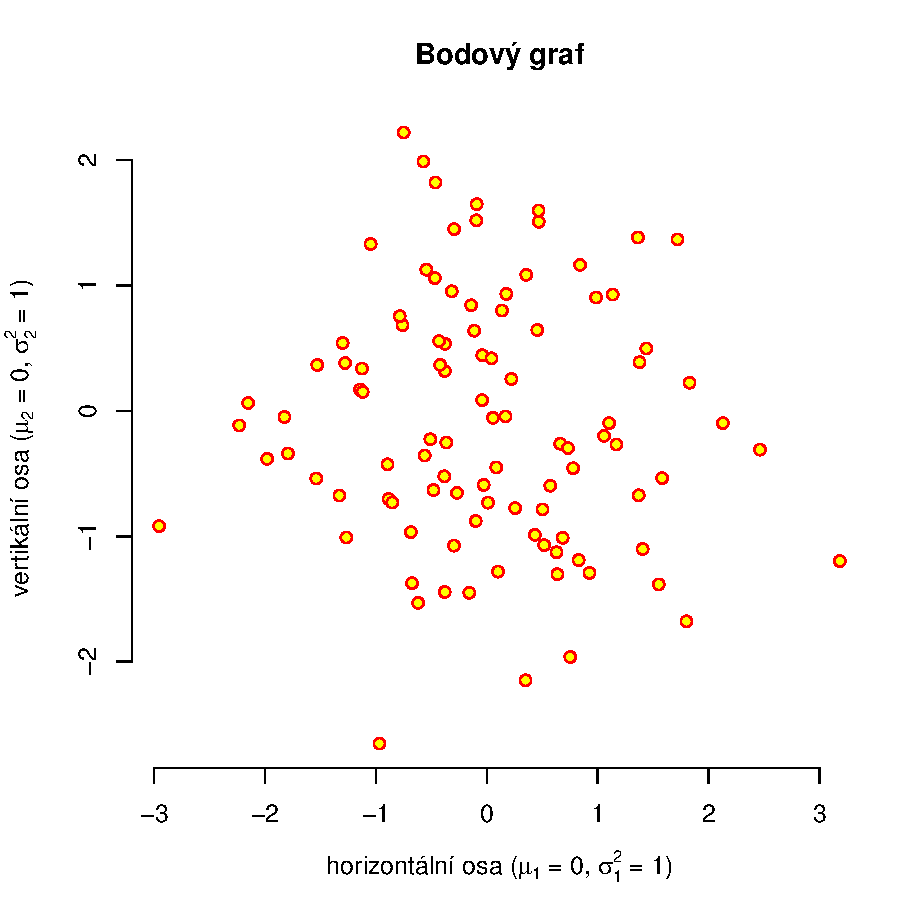
\includegraphics[width=.525\textwidth]{img/ukazka-obr01}
% Příponu není potřeba explicitně uvádět, pdflatex automaticky hledá pdf.
% Rozměry také není nutné uvádět.
\end{center}

\footnotesize \textit{Poznámka:} 
Vlastní zpracování na základě dat z ČSÚ.
\end{figure}

Několik rad týkajících se obrázků a grafů.

\begin{itemize}
\item Graf by měl být vytvořen ve velikosti, v~níž bude použit
  v~práci. Zmenšení příliš velkého grafu vede ke špatné čitelnosti
  popisků.
\item Osy grafu musí být řádně popsány ve stejném jazyce, v~jakém je
  psána práce (absenci diakritiky lze tolerovat). Kreslíme-li graf
  hmotnosti proti výšce, nenecháme na nich popisky \texttt{ht} a
  \texttt{wt}, ale osy popíšeme \emph{Výška [cm]} a~\emph{Hmotnost
    [kg]}. Kreslíme-li graf funkce $h(x)$, popíšeme osy $x$ a $h(x)$.
  Každá osa musí mít jasně určenou škálu.
\item Chceme-li na dvourozměrném grafu vyznačit velké množství bodů,
  dáme pozor, aby se neslily do jednolité černé tmy. Je-li bodů mnoho,
  zmenšíme velikost symbolu, kterým je vykreslujeme, anebo vybereme
  jen malou část bodů, kterou do grafu zaneseme. Grafy, které obsahují
  tisíce bodů, dělají problémy hlavně v~elektronických dokumentech,
  protože výrazně zvětšují velikost souborů.
\item Budeme-li práci tisknout černobíle, vyhneme se používání barev.
  Čáry roz\-li\-šu\-je\-me typem (plná, tečkovaná, čerchovaná,\ldots), plochy
  dostatečně roz\-díl\-ný\-mi intenzitami šedé nebo šrafováním. Význam
  jednotlivých typů čar a~ploch vysvětlíme buď v~textové legendě ke
  grafu anebo v~grafické legendě, která je přímo součástí obrázku.
\item Vyhýbejte se bitmapovým obrázkům o~nízkém rozlišení a zejména
  JPEGům (zuby a kompresní artefakty nevypadají na papíře pěkně).
  Lepší je vytvářet obrázky vektorově a vložit do textu jako PDF.
\end{itemize}


\section{Tabulky}

Pro vkládání tabulek použivejte plovoucí prostředí \verb|table| a navíc:
\begin{itemize}
\item pro popisky slouží příkaz \verb|\caption| -- umisťuje se pak také do seznamu tabulek,
\item příkaz \verb|\caption| se umisťuje se nad tabulku,
\item k identifikaci tabulky slouží příkaz \verb|\label| (musí být vždy za příkazem \verb|\caption|) -- na tabulku se v textu pak odkazujte příkazem \verb|\ref|,
\item zdroj a případné poznámky nebo legenda se umisťují pod tabulku, text není nijak zvýrazněn.
\end{itemize}

\begin{table}[htbp!]

\begin{center}
%%% Tabulka používá následující balíčky:
%%%   - booktabs (\toprule, \midrule, \bottomrule)
%%%   - dcolumn (typ sloupce D: vycentrovaná čísla zarovnaná na
%%%     desetinnou čárku
%%%     Všimněte si, že ve zdrojovém kódu jsou desetinné tečky, ale
%%%     tisknou se čárky.

\caption{Maximálně věrohodné odhady modelů 1 a 2}\label{tab03:Nejaka}
\begin{tabular}{lrr}
\toprule
              & \multicolumn{1}{c}{\textbf{1}} & \multicolumn{1}{c}{\textbf{2}}\\
\midrule
\multirow{2}{*}{Abs. člen}     &$-10,01$***  &42,01**\\
                               & (1,01)      &(1,89)\\
\multirow{2}{*}{Pohlaví (muž)} &	9,89*       & 8,16\\
                               & (5,98)	    &(8,18)\\
Výška (cm)                	   & 0,78***     &(0,12)	\\
\bottomrule
\end{tabular}
\end{center}

\footnotesize \textit{Poznámka:} 
(i) V závorkách jsou uvedeny směrodatné chyby získané na základě 500 iterací neparametrického bootstrapu.\\
(ii) * p < 0,05, ** p < 0,01, *** p < 0,001.\\
(iii) Vlastní zpracování na základě dat z ČSÚ.
\end{table}

U~\textbf{tabulek} se doporučuje dodržovat následující pravidla:

\begin{itemize} %% nebo compactitem z balíku paralist
\item Vyhýbat se svislým linkám. Silnějšími vodorovnými linkami
  oddělit tabulku od okolního textu včetně legendy, slabšími
  vodorovnými linkami oddělovat záhlaví sloupců od těla tabulky a
  jednotlivé části tabulky mezi sebou. V~\LaTeX u tuto podobu tabulek
  implementuje balík \texttt{booktabs}. Chceme-li výrazněji oddělit
  některé sloupce od jiných, vložíme mezi ně větší mezeru.
\item Neměnit typ, formát a význam obsahu buněk v~tomtéž sloupci
  (není dobré do téhož sloupce zapisovat tu průměr, jinde procenta).
\item Všechna čísla jsou uvedena s přesností na stejný počet platných číslic. Čísla v tabulce zarovnávat na desetinnou čárku.
\item K formátování hodnot obecně:
	\begin{itemize}
  \item Číselná data jsou v buňkách zarovnána doprava. 
  \item Texty umístěné v buňkách tabulky jsou zarovnány doleva nebo na střed, slova se nedělí..
	\end{itemize}
\item V~tabulce je někdy potřebné používat zkratky, které se jinde
nevyskytují. Tyto zkratky můžeme vysvětlit v~legendě nebo
v~poznámkách pod tabulkou. Poznámky pod tabulkou můžeme využít i
k~podrobnějšímu vysvětlení významu  některých sloupců nebo hodnot.
\end{itemize}


\section{Zdrojové kódy}
Algoritmy, výpisy programů a popis interakce s~programy je vhodné odlišit od ostatního textu. Jednou z~možností je použití {\LaTeX}o\-vé\-ho balíčku \texttt{listings} a jeho prostředí \texttt{lstlistings}.

V~souboru \texttt{makra.tex} je nadefinováno prostředí \texttt{code}. Jeho použití vypadá takto:
\begin{verbatim}
\begin{code}{programovací-jazyk}{popisek}{label}
import numpy as np
    
def incmatrix(genl1,genl2):
...
\end{code}
\end{verbatim}

\noindent
Například výpis \ref{zpracovani-python} je vložen takto:
\begin{verbatim}
\begin{code}{Python}{Ukázka zpracování pomocí Pythonu}{zpracovani-python}
...
\end{code}
\end{verbatim}

\begin{code}{Python}{Ukázka zpracování pomocí Pythonu}{zpracovani-python}
import numpy as np
    
def incmatrix(genl1,genl2):
    m = len(genl1)
    n = len(genl2)
    M = None #to become the incidence matrix
    VT = np.zeros((n*m,1), int)  #dummy variable
    
    #compute the bitwise xor matrix
    M1 = bitxormatrix(genl1)
    M2 = np.triu(bitxormatrix(genl2),1) 

    for i in range(m-1):
        for j in range(i+1, m):
            [r,c] = np.where(M2 == M1[i,j])
            for k in range(len(r)):
                VT[(i)*n + r[k]] = 1;
                VT[(i)*n + c[k]] = 1;
                VT[(j)*n + r[k]] = 1;
                VT[(j)*n + c[k]] = 1;
                
                if M is None:
                    M = np.copy(VT)
                else:
                    M = np.concatenate((M, VT), 1)
                
                VT = np.zeros((n*m,1), int)
    
    return M
\end{code}

Balíček \texttt{listings} a jeho prostředí \texttt{lstlisting} však nabízí téměř nepřeberné množství konfiguračních parametrů, např. pro zvýrazňování syntaxe programovacích jazyků (několika desítek), číslování řádku atd. Příklady:
\begin{itemize}
\item \url{https://en.wikibooks.org/wiki/LaTeX/Source_Code_Listings}
\item \url{https://www.overleaf.com/learn/latex/Code_listing#Using_listings_to_highlight_code}
\end{itemize}


\section{Sazba matematiky}
Proměnné sázíme kurzívou (to \TeX{} v~matematickém módu dělá sám, ale
nezapomínejte na to v~okolním textu a také si matematický mód zapněte).
Názvy funkcí sázíme vzpřímeně. Tedy například:
$\textrm{var} (X) = \textsf{E~} X^2 - \bigl(\textsf{E~} X \bigr)^2$.

Zlomky uvnitř odstavce (třeba $\frac{5}{7}$ nebo $\frac{x+y}{2}$) mohou
být příliš stísněné, takže je lepší sázet jednoduché zlomky s~lomítkem:
$5/7$, $(x+y)/2$.

Pro méně obeznámené se zvyklostmi v matematické sazbě lze doporučit stručný text od Richarda Starého -- \url{http://richardstary.wz.cz/clanky/matsaz/matsaz.pdf} --, který je obecně platný bez ohledu na to, zda použijete \LaTeX\ nebo Word.

Možnosti \LaTeX u pro sazbu matematiky jsou sice bohaté, ale je možné, že v některých specifických situacích nebudou postačovat. Proto lze doporučit k použití balíčky American Mathematical Society (AMS). V souboru \texttt{makra.tex} jsou standardně zaváděny balíčky \texttt{amsmath}, \texttt{amsfonts} a \texttt{amsthm}. Pro proniknutí do jejich možností poslouží:
\begin{itemize}
\item Math Extension with AMS\LaTeX\ -- \url{http://ptgmedia.pearsoncmg.com/images/0321173856/samplechapter/kopkach15.pdf}
\item \url{https://www.overleaf.com/learn/latex/Aligning_equations_with_amsmath}
\item Math Mode -- \url{http://tex.loria.fr/general/Voss-Mathmode.pdf}
\item More Math into LaTeX -- \url{http://tug.ctan.org/info/Math_into_LaTeX-4/Short_Course.pdf}
\end{itemize}

Ukázka číslovaného vzorce:
\begin{equation}
\mathbf{b}=(\mathbf{X}^\mathsf{T}\mathbf{X})^{-1}\mathbf{X}^\mathsf{T}\mathbf{y}
\end{equation}

Ukázka nečíslovaných vzorců s funkcemi a indexy:

$$
d_{ij}=\max_{k=1,2,\dots,n} \{d_{ik}+d_{kj}\},
$$
$$
x_{1,2}=b \pm \sqrt{\ln y}.
$$

Ukázku vzorce jako součást jednoho odstavce uveďme na příkladu kapacit dodavatelů v matematickém modelu dopravního problému, které zohledníme pomocí omezení:
\begin{equation}
\sum_{j=1}^n x_{ij} \le a_i, \qquad i=1,2,\dots,m\ ,
\end{equation}
\noindent
kde výraz $a_i$ představuje kapacitu $i$-tého dodavatele.

Při odvozování vzorce postupnou úpravou se obvykle jednotlivé kroky uvádějí na samostatných řádcích (prostředí \verb'align*' z balíčku \verb|amsmath|):
\begin{align*}
 f(x) &= (x+a)(x+b) =\\
      &= x^2 + bx + ax + ab =\\
      &= x^2 + (a+b)x + ab
\end{align*}

Ukázka sloupcové úpravy (\verb|eqnarray*|):
\begin{eqnarray*}
\sum_{i=1}^n x_{ij} =1, && j=1,2,\dots,n,\\
\sum_{j=1}^n x_{ij} =1, && i=1,2,\dots,n,\\
u_i + 1 - M(1 - x_{ij}) \le u_j, && i=2,3,\dots,n,\quad j=1,2,\dots,n,\\
u_i \ge 0,              && i=1,2,\dots,n,\\
x_{ij} \in \{0,1\} && i=1,2,\dots,n,\quad j=1,2,\dots,n,\\
\end{eqnarray*}
% %%% Fiktivní kapitola s ukázkami citací

\chapter{Práce s literaturou}

\lettrine[lines=2]{!}{~}\textbf{V seznamu literatury se uvádějí pouze zdroje, na které se v textu práce odkazuje ve formě parafrází nebo přímých citací.}

Tato šablona předpokládá použití bibliografické databáze ve formátu \BibTeX\ z důvodu větší flexibility. Použití bibliografické databáze není nutnou podmínkou, lze si vystačit i se standardním prostředím \texttt{thebibliography}. V takovém případě je však zapotřebí provést zásahy do některých souborů, jak je uvedeno dále.

\section{Použití bibliografické databáze}

\begin{enumerate}
\item \textbf{Balíček \verb'biblatex', APA-7}\\
Šablona využivá pro zpracování bibliografické databáze nastavení přes balíček \verb|biblatex| a rovněž garantuje použití citačního standardu \textbf{APA-7}. Veškerá nastavení jsou uvedena v souboru \texttt{biblatex-setup.tex}.
\item\textbf{Změna názvu databáze}\\
V šabloně se předpokládá databáze uložená v souboru \texttt{literatura.bib}. Pokud se databáze jmenuje jinak, pak je nutné v souboru \texttt{biblatex-setup.tex} změnit hodnotu parametru příkazu \verb'\bibliography'.
\item\textbf{Změna citačního stylu}\\
Standardně se citace v textu uvádějí v kombinaci příjmení a roku (harvardský styl). Lze přepnout i na odkazy číslem změnou v souboru \texttt{biblatex-setup.tex}, kde se zruší komentářový znak v řádcích:
\begin{verbatim}
%  ,citestyle=numeric-comp
...
%\makeatletter
%\RequireBibliographyStyle{numeric}
%\makeatother
\end{verbatim}
\item \textbf{Využití populárního citačního manažeru Zotero}:
\begin{enumerate}
\item více informací -- \href{https://www.zotero.org/}{homepage}, \href{https://knihovna.vse.cz/citace/nastroje/zotero/}{informace z Knihovny VŠE}
\item Instalace -- \url{https://www.zotero.org/download/}
\item Instalace konektoru do prohlížeče -- Firefox, Chrome, Edge, Safari
\item Rozšíření Better BibTeX for Zotero -- \url{https://retorque.re/zotero-better-bibtex/}:
     \begin{enumerate}
     \item Stáhnout .xpi soubor
     \item A pak \texttt{Nástroje--Doplňky--Instal Add-on From File}
     \end{enumerate}
\item \href{https://formadoct.doctorat-bretagneloire.fr/zotero_workshop/latex}{Zotero workshop aneb Zotero\&{}\LaTeX\ krok po kroku}
\end{enumerate}
\end{enumerate}


\section{Použití prostředí \texttt{thebibliography}}
\begin{enumerate}
\item V souboru \texttt{makra.tex} vymazat na počátku tyto řádky:
\begin{verbatim}
%%% Nastavení pro použití samostatné bibliografické databáze.
%%% Settings for using a separate bibliographic database.
\input biblatex-setup
\end{verbatim}
\item V souboru \texttt{literatura.tex} odstranit řádek s příkazem \verb'\printbibliography' a odstranit příznak komentáře v další části obsahující prostředí \texttt{thebibliography.}
\item Jednotlivé položky \verb\bibitem\ musí být sestaveny dle standardu APA-7. Návodné příklady jsou k dispozici třeba zde: \url{https://knihovna.vse.cz/citace/priklady/?norm=apa}.
\end{enumerate}


\section{Jak citovat v textu}
\begin{center}
\begin{tabularx}{\textwidth}{l@{~~$\longrightarrow$~~}X}
\verb|\parencite{Cermak2018}|&\parencite{Cermak2018}\\
nebo \verb|\cite{Cermak2018}|&\cite{Cermak2018}\\
\verb|\parencite{Hladik2018,Jasek2018}|&\parencite{Hladik2018,Jasek2018}\\
\verb|\parencite[kap. 3]{Pecakova2018}|&\parencite[kap. 3]{Pecakova2018}\\
\verb|\parencite{Furtuna2023}|&\parencite{Furtuna2023}\\
\verb|\parencite{shanahan2024talking}|&\parencite{shanahan2024talking}\\
\end{tabularx}
\end{center}

% %%% Fiktivní kapitola s instrukcemi k PDF/A

\chapter{Formát PDF/A}

Elektronická podoba závěrečných
prací musí být odevzdávána ve formátu PDF/A úrovně 1a nebo 2u. To jsou
profily formátu PDF určující, jaké vlastnosti PDF je povoleno používat,
aby byly dokumenty vhodné k~dlouhodobé archivaci a dalšímu automatickému
zpracování. Dále se budeme zabývat úrovní 2u, kterou sázíme \TeX{}em.

Mezi nejdůležitější požadavky PDF/A-2u patří:

\begin{itemize}

\item Všechny fonty musí být zabudovány uvnitř dokumentu. Nejsou přípustné
odkazy na externí fonty (ani na \uv{systémové}, jako je Helvetica nebo Times).

\item Fonty musí obsahovat tabulku ToUnicode, která definuje převod z~kódování
znaků použitého uvnitř fontu to Unicode. Díky tomu je možné z~dokumentu
spolehlivě extrahovat text.

\item Dokument musí obsahovat metadata ve formátu XMP a je-li barevný,
pak také formální specifikaci barevného prostoru.

\end{itemize}

Tato šablona používá balíček {\tt pdfx,} který umí \LaTeX{} nastavit tak,
aby požadavky PDF/A splňoval. Metadata v~XMP se generují automaticky podle
informací v~souboru {\tt prace.xmpdata} (na vygenerovaný soubor se můžete
podívat v~{\tt pdfa.xmpi}).

Správnost PDF/A lze zkontrolovat pomocí on-line validátoru: \url{https://www.pdf-online.com/osa/validate.aspx/}.

Pokud soubor nebude validní, mezi obvyklé příčiny patří používání méně
obvyklých fontů (které se vkládají pouze v~bitmapové podobě a/nebo bez
unicodových tabulek) a vkládání obrázků v~PDF, které samy o~sobě standard
PDF/A nesplňují.

Je pravděpodobné, že se to týká obrázků vytvářených mnoha různými programy.
V~takovém případě se můžete pokusit obrázek do zkonvertovat do PDF/A pomocí
GhostScriptu, například takto:

\begin{verbatim}
        gs -q -dNOPAUSE -dBATCH
           -sDEVICE=pdfwrite -dPDFSETTINGS=/prepress
           -sOutputFile=vystup.pdf vstup.pdf
\end{verbatim}

\chapter{Teoreticko-metodologická východiska}
Tato kapitola poskytuje teoretický a metodologický rámec nezbytný pro analýzu a redesign uživatelského rozhraní aplikace. Jejím cílem je představit základní pojmy, principy a trendy v oblasti workplace management software, UX a UI designu, design systémů a evaluace použitelnosti. Součástí kapitoly je rovněž přehled metod a nástrojů, které slouží k identifikaci problémů současného rozhraní a k návrhu optimálního, uživatelsky přívětivého řešení. Teoretická východiska poskytují nezbytný kontext pro praktickou část práce a umožňují aplikovat osvědčené postupy při systematickém redesignu aplikace.

\section{Workplace management software}
% Tuto podkapitolu jsem pro toto zadání přeskočil, ale ve finální diplomové práci jí chci mít přibližně na tomto místě.

\section{UX a UI design}
V oblasti digitálních produktů se pojmy UX (User Experience/Uživatelský zážitek) design a UI (User Interface/Uživatelské rozhraní) design stal klíčovým pro vytváření efektivních a intuitivních rozhraní. UX design je disciplína zaměřující se na řízení celkové zkušenost uživatele při používání nějaké aplikace. UI design je disciplína zaměřující se na vizuální stránku prvků rozhraní.

\subsection{Principy UX designu}
Hlavním cílem UX designu je zajistit, aby uživatelé mohli efektivně, intuitivně a bez zbytečné mentální námahy dosáhnout svých cílů. Podle Dona Normana (Norman, 2013) lze klíčové pricipy UX designu shrnout následovně
\begin{itemize}
    \item Orientace na uživatele (user-centered design) – návrh je založen na potřebách uživatelů
    \item Použitelnost (usability) – ovládání produktu má být snadno naučitelné a jednoduché na používání
    \item Předvídatelnost – prvky a interakce napříč aplikací musí mít jednotný vzhled a chování
    \item Viditelná zpětná vazba – informování uživatele o provedené změně, úspěchu či chybě
    \item Minimalizace kognitivní zátěže – rozhraní by mělo být přehledné, intuitivní a logicky strukturované
\end{itemize}


\subsection{Principy UI designu}
UI design se zaměřuje na vizuální a interakční stránku rozhraní.
\begin{itemize}
    \item Jasná vizuální hierarchie – klíčové prvky jsou zvýrazněny a vedou uživatele logickým způsobem
    \item Konzistence a standardizace – opakující se prvky mají stejný vzhled a stejné chování
    \item Minimalismus a jednoduchost – odstranit nepotřebné prvky, aby rozhraní bylo přehledné
    \item Interakční zpětná vazba – animace, změny barev nebo stavů indikují, že systém reaguje na akce uživatele
\end{itemize}
UI design v praxi úzce souvisí s UX, protože vizuální a interakční prvky ovlivňují, jak snadno a příjemně uživatelé dosahují svých cílů. (Dannaway, 2024)

\subsection{Heuristické zásady}
Heuristická evaluace představuje expertní metodu posuzování rozhraní podle osvědčených principů použitelnosti. Jacob Nielsen (1994) definoval deset základních heuristik, které se často používají při hodnocení a redesignu komplexních aplikací.
\begin{enumerate}
    \item Viditelnost stavu systému
    \item Shoda mezi systémem a reálným světem
    \item Uživatelská kontrola a svoboda
    \item Konzistence a standardy
    \item Prevence chyb
    \item Rozpoznání místo vybavování
    \item Flexibilita a efektivita použití
    \item Estetický a minimalistický design
    \item Pomoc při chybách
    \item Nápověda a dokumentace
\end{enumerate}
Použití heuristických principů je při redesignu stávajících modulů aplikace zásadní pro odhalení nekonzistentních prvků, problémové navigace a oblastí s vysokou kognitivní zátěží.

\section{Design systémy}
Design systémy představují v současnosti jeden z nejdůležitějších nástrojů při návrhu a vývoji digitálních produktů. Reagují na potřebu dlouhodobé konzistence, škálovatelnosti a efektivní spolupráce mezi designéry a vývojáři, zejména v případech rozsáhlých nebo dynamicky se rozvíjejících aplikací. V situaci, kdy produkty obsahují desítky až stovky obrazovek či modulů, se design systém stává klíčovým prvkem umožňujícím udržet jednotnou vizuální a interakční logiku. (Kholmatova, 2017)

\subsection{Definice a účel design systému}
Podle Ally Kholmatové neexistuje žádná jednotná, univerzálně přijímaná definice design systému. V knize Design Systems definuje design systém jako soubor vzájemně propojených vzorů a sdílených postupů, které jsou koherentně uspořádány za účelem podpory digitálních produktů.
Vzory jsou opakující se prvky, které kombinujeme při tvorbě rozhraní. Jde například o uživatelské toky, interakce, tlačítka, formulářová pole, ikony, barvy, typografie nebo microcopy (krátké texty).
Postupy pak znamenají to, jakým způsobem budeme tyto vzory vytvářet, zaznamenávat, sdílet, a používat. Zejména při týmové spolupráci. (Kholmatova, 2017)
Design systém podle zmíněné definice spojuje tři základní roviny
\begin{itemize}
    \item Vizuální prvky – definice estetické podoby zobrazení
    \item Komponentový systém – katalog prvků určených k opakovanému použití
    \item Pravidla a procesy – metodika, jak se jednotlivé prvky používají, kombinují a rozvíjejí
\end{itemize}
Primárním účelem design systému je vytvořit jednotnou a konzistentní uživatelskou zkušenost napříč aplikací, modulární strukturu podporující efektivní vývoj a snížení chybovosti způsobené nesourodostí stylů či komponent.

\subsection{Principy design systémů}
Jedním z nejrozšířenějších přístupů k tvorbě design systémů je Atomic Design, který představil Brad Frost (2016). Tento model dělí uživatelské rozhraní do pěti úrovní
\begin{enumerate}
    \item Atomy – základní prvky jako barvy, typografické styly, ikony či jednoduché UI prvky
    \item Molekuly – kombinace atomů (např. input + ikona)
    \item Organismy – větší komponenty (např. hlavička stránky)
    \item Šablony – strukturální kostra obrazovek
    \item Stránky – konkrétní realizace šablon s reálným obsahem
\end{enumerate}
Tento přístup usnadňuje škálování designu, protože změna na nízké úrovni (např. úprava barevného tokenu) se může automaticky promítnout v celém systému.

\subsection{Přínosy design systémů}
Podle studií společnosti Sparkbox, která prováděla průzkumy Design Systems Survey každý rok mezi lety 2018 až 2022, dokáže organizace s funkčním design systémem zkrátit čas tvorby obrazovek až o 50 %. Další výhody zahrnují
\begin{itemize}
    \item Rychlejší vývoj – vývojáři opakovaně používají již schválené komponenty místo vytváření nových
    \item Snížení technického dluhu – díky jednotné knihovně komponent se eliminuje nekonzistence a potřeba předělávek
    \item Lepší komunikace v týmu – designéři, vývojáři a produktoví manažeři pracují se stejným pojmovým rámcem
    \item Snazší onboarding nových členů – noví designéři a vývojáři se rychleji orientují ve vizuálním jazyce produktu
    \item Vyšší kvalita UX – repetitivní používání testovaných komponent vede k menší chybovosti uživatelů a vyšší spokojenosti (Sparkbox, n. r.)
\end{itemize}
    

% \subsection{Design systém}
% Software musí splňovat vyšší nároky na profesionální vizuální identitu, intuitivnost a očekávání zákazníků. Dhanwani (2025) uvádí, že moderní B2B produkty jsou hodnoceny nejen podle funkcionality, ale především podle kvality uživatelské zkušenosti – a design systém je jedním z hlavních nástrojů, jak tuto kvalitu zajistit.
% Design systém umožní
% •	efektivní přidávání nových modulů bez ztráty konzistence
% •	snazší přizpůsobení produktu specifickým požadavkům klientů
% •	budování vizuální identity podporující důvěru v produkt
% •	dlouhodobě udržitelný rozvoj bez návratu k chaotickému organickému růstu

\section{Metody použitelnosti a evaluace}
Uživatelský výzkum, testování použitelnosti, vhodné metody
\chapter{Analýza současného stavu aplikace}

\section{Historie a vývoj aplikace}
Kontext vzniku během pandemie, postupné rozšiřování modulů, hlavní funkce a jejich charakteristika

\section{Analýza uživatelského rozhraní}
Heuristické posouzení, identifikace nekonzistencí a problémových míst, posouzení vizuální hierarchie, navigace, ovládacích prvků

\section{Uživatelský výzkum a zpětná vazba}
Metodika sběru dat, shrnutí hlavních problémů identifikovaných uživateli, dopad problémů na efektivitu práce

\section{Vstupní požadavky pro redesign}
Interní a legislativní požadavky, požadavky související s komercializací, technická omezení a příležitosti

\chapter{Design systém a vizuální identita}

\section{Definice vizuální koncepce}
Barevná paleta, typografie, ikonografie a ilustrace

\section{Tvorba komponent}
Tlačítka, inputy, tabulky, kalendáře, karty, modální okna, stavové varianty, přístupnost, responsivita

\section{Dokumentace a pravidla používání}
Guidelines pro návrháře i vývojáře, pravidla pro rozšiřování systému, sjednocení stylu napříč aplikací

\chapter{Redesign vybraných modulů}
TODO: Tvorba prototypů obrazovek v nástroji Figma
\chapter{Evaluace navrženého řešení}

\section{Metodika testování}
TODO: Popis testovacího scénáře, výběr uživatelů

\section{Výsledky uživatelského testování}
TODO: Identifikované problémy, silné stránky nového návrhu

\section{Interpretace výsledků a zapracování změn}
TODO: Návrhy úprav podle zpětné vazby, porovnání s výchozím stavem
\chapter{Doporučení pro další rozvoj}

TODO: Následná buducí implementace, rozšiřování modulů pomocí design systému, návrhy pro kontinuální výzkum a evaluaci
{%
\pagestyle{plain}
\chapter*{Závěr}
\addcontentsline{toc}{chapter}{Závěr}

% Shrnutí cílů a jejich naplnění, přínosy redesignu pro organizaci i budoucí zákazníky, reflexe postupu a metod, možnosti pokračování projektu

V rámci diplomové práce se podařilo úspěšně navrhnout a na uživatelích ověřit nový uživatelský design aplikace pro správu pracovního prostředí. S využitím metod uživatelsky orientovaného designu byl vytvořen komplexní návrh, který je nyní připraven k technické implementaci.

Během řešení práce byly zodpovězeny všechny stanovené výzkumné otázky:

\begin{itemize}
    \item \textbf{K otázce hlavních bariér v použitelnosti (VO1)} analýza a výzkum ukázaly, že uživatelé nejvíce naráželi na nekoherentní navigaci, absenci logické vizuální hierarchie a roztříštěnost ovládacích prvků napříč různými moduly, které vznikaly organicky a bez jednotného zadání.
    \item \textbf{Pro zajištění vizuální konzistence a budoucího škálování (VO2)} byl vytvořen ucelený design systém. Tento systém definuje nejen základní vizuální styl, ale funguje jako standardizovaná knihovna komponent, která umožní vývojovému týmu efektivně přidávat nové funkcionality bez narušení jednotného vzhledu a chování aplikace.
    \item \textbf{Zhodnocení vlivu redesignu na kognitivní zátěž (VO3)} proběhlo prostřednictvím uživatelského testování interaktivních prototypů. Výsledky testování použitelnosti jasně prokázaly, že nové rozhraní výrazně zvyšuje intuitivnost používání – uživatelé dokončovali zadané úkoly rychleji, s menší chybovostí a subjektivně vnímali práci se systémem jako méně zatěžující.
\end{itemize}

Výstupem diplomové práce je soubor vzájemně provázaných artefaktů, které naplňují definované cíle: výzkumná zpráva shrnující úvodní analýzu, ucelený design systém, interaktivní prototypy redesignovaných klíčových obrazovek připravené k implementaci, report o testování použitelnosti a grafický manuál definující metodický rámec pro další rozvoj.

Přínosem práce je vytvoření robustního a testováním ověřeného základu, který transformuje funkčně orientovaný interní nástroj do podoby moderního, přehledného a škálovatelného produktu. Z hlediska budoucího rozvoje se doporučuje bezproblémové předání (hand-off) vytvořených artefaktů vývojovému týmu k implementaci. Následný výzkum by se měl zaměřit na sběr kvantitativních dat z reálného provozu a případné rozšíření design systému o pokročilé standardy digitální přístupnosti.

}

%%% Seznam použité literatury
%% Toto platí v případě použití samostatné bibliografické databáze
\printbibliography[title={\bibnamex},heading={bibintoc}]

%% Toto platí v případě použití prostředí thebibliography
%% Pro sestavení citačních údajů lze doporučit:
%%     https://knihovna.vse.cz/citace/priklady/
%%     https://www.citace.com/
%\openright
%\phantomsection
%\addcontentsline{toc}{chapter}{\bibnamex}
%\begin{thebibliography}{99}
%\bibitem{Cermak2018}Čermák, R., \& Smutný, Z. (2018). A Framework for Cultural Localization of Websites and for Improving Their Commercial Utilization. In \textit{Global Observations of the Influence of Culture on Consumer Buying Behavior} (s. 206–-232). IGI Global. https://doi.org/10.4018/978-1-5225-2727-5.ch013
%\bibitem{Furtuna2023}Furtună, T. F., Vint,e, C., \& Proscanu, C. (2023). Interchanging Java–Python Data with Applications in Machine Learning Solutions. 321, 329–-342.
%\bibitem{Hladik2018}Hladík, M., \& Černý, M. (2018). The Shape of the Optimal Value of a Fuzzy Linear Programming Problem. \textit{Fuzzy Logic in Intelligent System Design}, 281–-286. https://doi.org/10.1007/978-3-319-67137-6\_31
%\bibitem{Jasek2018}Jašek, P., Vraná, L., Šperková, L., Smutný, Z., \& Kobulský, M. (2018). Modeling and Application of Customer Lifetime Value in Online Retail. \textit{Informatics}, 5(1). http://www.mdpi.com/2227-9709/5/1/2/pdf
%\bibitem{Pecakova2018}Pecáková, I. (2018). \textit{Statistika v terénních průzkumech}. Professional Publishing.
%\end{thebibliography}


%%% Přílohy k práci, existují-li. Každá příloha musí být alespoň jednou
%%% odkazována z vlastního textu práce. Přílohy se číslují.
\part*{\Prilohy\thispagestyle{empty}}
\appendix
\chapter{Název první přílohy}


\chapter{Název druhé přílohy}


% \include{...}
% \include{...}

\end{document}